\documentclass{article}
\usepackage{graphicx}
\usepackage[utf8]{inputenc}
\usepackage{listings}
\usepackage{color}
\usepackage{xcolor}
\usepackage{textcomp}

\begin{document}

\title{Tarea Lagrange}
\author{Angel Caceres Licona}

\maketitle


\section{Construya los polinomios interpolantes...}
\subsection{Para la función $\cos(x)$}
Para el polinomio de 1er grado obtenemos: 
$$L(x)=1-0.291107x$$
Para el polinomio de 2o grado obtenemos: 
$$L(x)=-0.431087 x^2-0.0324551 x+1$$
Tenemos los siguientes valores:

\begin{center}
    \begin{tabular}{||c c||} 
    \hline
    $x$ & $f(x)$ \\ [0.5ex] 
    \hline
    0 & 1  \\ 
    \hline
    0.6 & 0.8253356 \\
    \hline
    0.9 & 0.6216099 \\
    \hline
   \end{tabular}
\end{center}

El valor real de la función en $x=0.45$ es: 0.9004471

El valor calculado usando el polinomio de grado 1 es: 0.8690018 con un error absoluto de 0.0314453

El valor calculado usando el polinomio de grado 2 es: 0.8981 con un error absoluto de 0.0023471

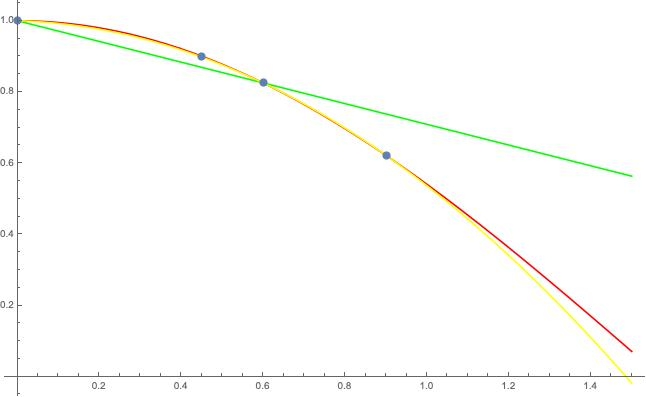
\includegraphics[scale=0.5]{Grafica1.jpeg}

\subsection{Para la función $\sqrt(1+x)$}
Para el polinomio de 1er grado obtenemos: 
$$L(x)=1 +0.441518 x $$
Para el polinomio de 2o grado obtenemos: 
$$L(x)=-0.0702289 x^2+0.483656 x+1$$
Tenemos los siguientes valores:

\begin{center}
    \begin{tabular}{||c c||} 
    \hline
    $x$ & $f(x)$ \\ [0.5ex] 
    \hline
    0 & 1  \\ 
    \hline
    0.6 & 1.26491106 \\
    \hline
    0.9 & 1.3784048 \\
    \hline
   \end{tabular}
\end{center}

El valor real de la función en $x=0.45$ es: 1.2041594

El valor calculado usando el polinomio de grado 1 es: 0.9486855 con un error absoluto de 0.2554739

El valor calculado usando el polinomio de grado 2 es: 1.2034238 con un error absoluto de 0.0007356

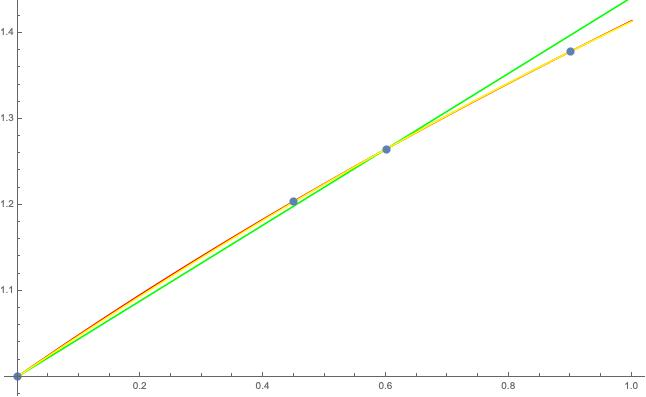
\includegraphics[scale=0.5]{Grafica2.jpeg}


\subsection{Para la función $\log(x+1)$}
Para el polinomio de 1er grado obtenemos: 
$$L(x)=0.783339 x$$
Para el polinomio de 2o grado obtenemos: 
$$L(x)=-0.233895 x^2+0.923676 x$$
Tenemos los siguientes valores:

\begin{center}
    \begin{tabular}{||c c||} 
    \hline
    $x$ & $f(x)$ \\ [0.5ex] 
    \hline
    0 & 0  \\ 
    \hline
    0.6 & 0.4700036 \\
    \hline
    0.9 & 0.6418538 \\
    \hline
   \end{tabular}
\end{center}

El valor real de la función en $x=0.45$ es: 0.37156355

El valor calculado usando el polinomio de grado 1 es: 0.3525025 con un error absoluto de 0.01906105

El valor calculado usando el polinomio de grado 2 es: 0.3682904 con un error absoluto de 0.00327315


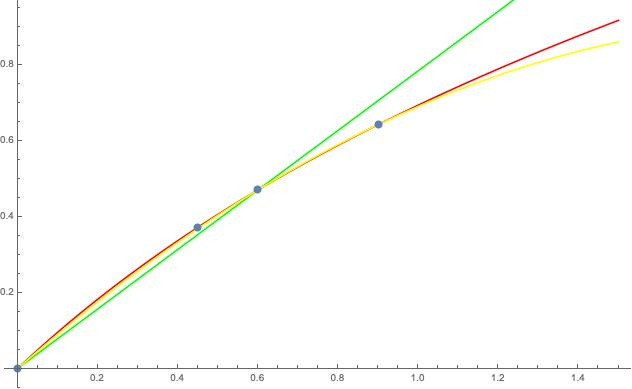
\includegraphics[scale=0.5]{Grafica3.jpeg}

\subsection{Para la función $\tan(x)$}
Para el polinomio de 1er grado obtenemos: 
$$L(x)=1.14023 x$$
Para el polinomio de 2o grado obtenemos: 
$$L(x)=0.866493 x^2+0.620332 x$$
Tenemos los siguientes valores:

\begin{center}
    \begin{tabular}{||c c||} 
    \hline
    $x$ & $f(x)$ \\ [0.5ex] 
    \hline
    0 & 0  \\ 
    \hline
    0.6 & 0.6841368 \\
    \hline
    0.9 & 1.2601582 \\
    \hline
   \end{tabular}
\end{center}
 
El valor real de la función en $x=0.45$ es: 0.483055

El valor calculado usando el polinomio de grado 1 es: 0.513104 con un error absoluto de 0.030049

El valor calculado usando el polinomio de grado 2 es: 0.4546142 con un error absoluto de 0.0284408

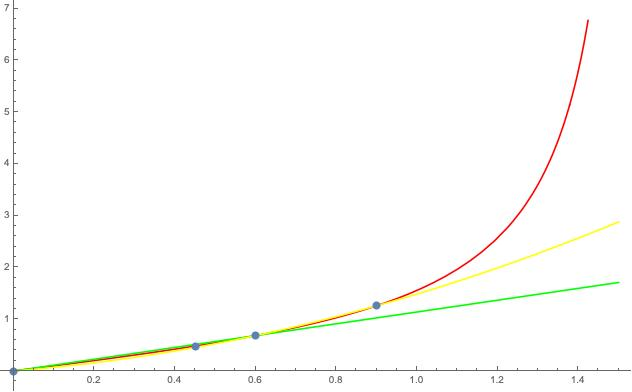
\includegraphics[scale=0.5]{Grafica4.jpeg}

\section{Usa polinomios para aproximar $f(8.4)$}

Para el primer polinomio tenemos: 
$$L(x) = 6.88682 + 1.24164 x$$

La aproximación que obtenemos es: 17.316596

Para el segundo polinomio tenemos
$$L(x) = -4.16531+2.1201 x+0.06 x^2 $$

La aproximación que obtenemos es: 17.87713

Para el tercer polinomio tenemos
$$L(x) = -2.96077+1.6862 x+0.112083 x^2-0.00208333 x^3$$

La aproximación que obtenemos es: 17.87708845568

\end{document}